\section{Motivation}

The success of \itercomp relies on having representative inputs for the target program to be optimized. If the developers cannot predict
what will be the typical usage of the application or that typical usage changes over time, then \itercomp might fail making the application
faster for the user.

\begin{figure}[t!]
    \centering
    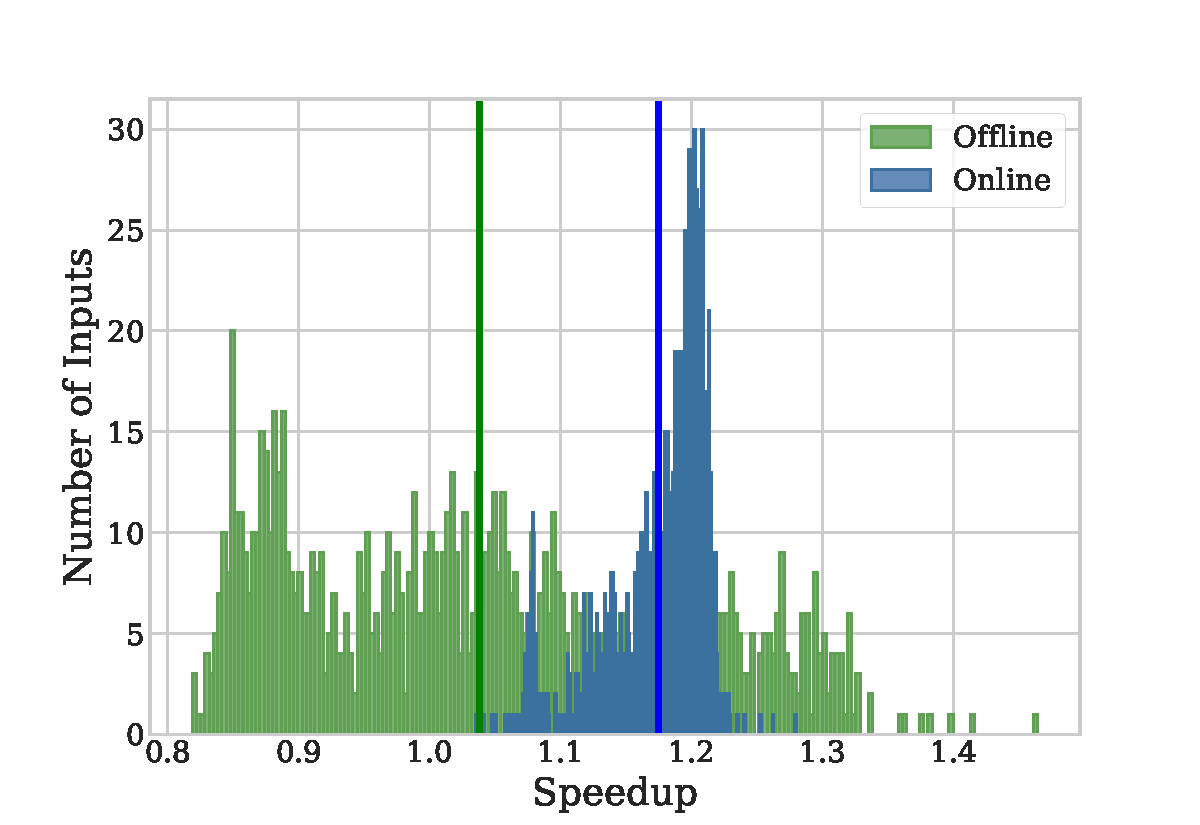
\includegraphics[width=0.5\textwidth]{figs/motivation-online.pdf}
    \caption{Histograms of speedup over \texttt{-O3} for each of the 1,000 inputs of \texttt{susan\_c}. The green histogram shows the speedup when using
    the optimization sequence selected by offline \itercomp, the blue one is the speedup using the optimization sequence selected by an
    online-like approach.}
    \label{fig:motivation-online}
\end{figure}

To show this, we performed offline \itercomp on \texttt{susan\_c} from the \textit{KDataSets} benchmark suit~\cite{chen10,chen12a} using a
small subset of its inputs to identify the best-performing optimization sequence. In Figure~\ref{fig:motivation-online}, the green bars are
the histogram of speedups compared to \red{LLVM?} \texttt{-O3} for each individual input, while the dark green line shows the speedup
averaged over all inputs. Despite the selected optimization sequence being the best for some inputs, we see that it delivers, on average,
6\% of performance improvement, but gives slows down performance for nearly of the inputs. This example shows that randomly choosing an
input set to use for offline \itercomp can be counterproductive.

The blue bars \red{zw: the reviewer won't be able to see the difference if the paper is printed in black and white.} in
Figure~\ref{fig:motivation-online} show a different approach where during \itercomp the speedup of each optimization sequence is again
measured on a small input subset but this subset changes for every optimization sequence. This is similar to how online \itercomp would
have to work, using each input only once. This might introduce errors, since the speedups we measure for each optimization sequence are not
strictly comparable, they are measured on different workloads. But in the end the histogram shows that being able to test more inputs
allows us to make better informed decisions. The optimization sequence we selected never degrades performance compared to \texttt{-O3} and
is on average 13\% better than the offline approach.

\begin{figure}[t]
    \centering
    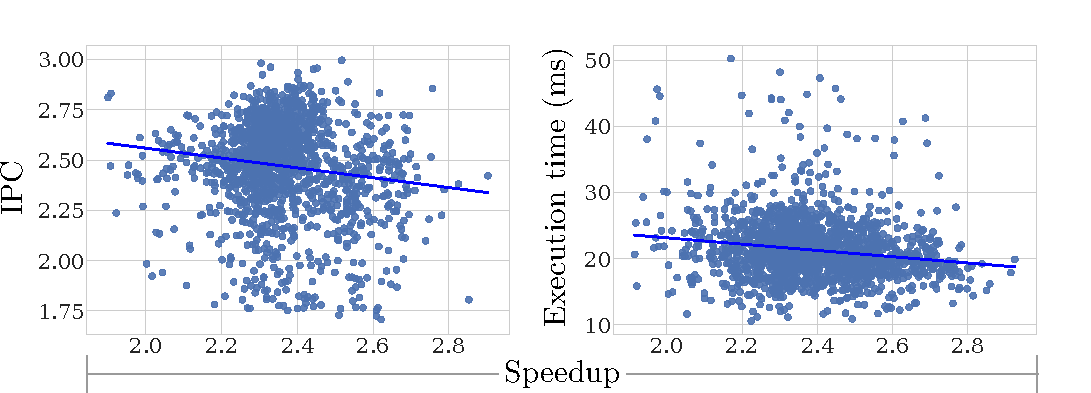
\includegraphics[width=0.5\textwidth]{figs/motivation-metric.pdf}
    \caption{Relationship between IPC and execution time vs optimization speedup for 500 different binaries of \texttt{susan\_c}. The binaries are compiled using different optimization sequences. Each point represents
	averages over a distinct subsets of its inputs.}
    \red{ZW: Perhaps take out the blue line (execution time). It is rather confusing. }
    \label{fig:motivation-metric}
\end{figure}

This is not an entirely surprising result. Evaluating our optimization decisions on more inputs decreases the chances of optimizing for an
unrepresentative input. Despite that offline \itercomp is still the preferred way. Measuring the speedup caused by an optimization requires
running the same input \textit{at least twice}, one of the optimized and one for the baseline binary. This is either infeasible or
undesirable in a realistic online \itercomp scenario. There are two existing workarounds to this problem: directly comparing the
\textit{execution time} of each run against previous runs or directly comparing the \textit{instructions per cycle}~(IPC)~\citep{fursin07}.
Neither metric is a good proxy for speedup. Figure~\ref{fig:motivation-metric} plots the measured IPC and execution time versus the real
speedup for 500 different binaries of the \texttt{susan\_c} benchmark. IPC, execution time, and speedup are averaged over distinct subsets of its inputs.
Both metrics have no direct correlation with speedup. Different inputs require a different amount of work which dominates the changes in execution time. IPC on
the other hand might improve with a more efficient binary but the opposite can also be true. For example,
replacing many one-cycle instructions by fewer multi-cycle instructions.
%inserting \texttt{NOP} statements will usually improve IPC.

In the remaining of this paper, we describe our work efficiency metric, which provides a new way for approximating optimization speedup
through a single run. We show that by utilizing this metric, a highly effective online \itercomp methodology can be built.

% %As a motivation example, consider...
%
% %Here we give an example to motivate our work. E.g. assuming we have a zero-cost profiling based work metric,
% %how can we use it to perform iterative compilation across runs? Then we talk about while it is impossible to
% %build a zero-overhead metric, we can develop one with low overhead.
%
% This section provides a comparison between the offline and online approaches for
% {\itercomp}.
% The goal is to motivate the need for an online {\itercomp}, highlighting
% weaknesses of using offline {\itercomp}.
%
% %In the offline approach, a fixed set of inputs is selected for which the best
% %optimization sequence is selected during the development time (pre-shipping) of
% %a program.
% %Although this fixed set of inputs is expected to be representative of the user's
% %workload,
% %in most cases, it might be infeasible to identify and collect representative
% %workloads for every group of users.
% %Furthermore, a user can dynamically change its workload pattern, rendering
% %a fixed optimization sequence innapropriate for his performance requirements.
%
% %In the online approach, the program is shipped with an initial optimization
% %sequence and different optimization sequences are evaluated as the end-user
% %executes the program.
% %This approach frees developers from the need to collect representative
% %workloads for every group of users so that the program can be optimized
% %accordingly.
% %More importantly, even in scenarios where the user's workload can dynamically
% %change its pattern, the online {\itercomp} would still be able to optimize the
% %program accordingly.
%
% In the offline approach, a small fixed set of inputs is selected for which all
% optimization sequences are evaluated.
% In the online approach, each optimization sequence is evaluated based on a,
% dynamically selected, distinct set of inputs.
% In both cases, the optimization sequences are ranked based on their average
% speedup, and the best optimization sequence is selected.
%
% In order to assess the quality of the optimization sequence selected by each
% approach, we evaluate both optimization sequences against all available inputs
% in our dataset.
% Figure~\ref{fig:motivation-online} shows this comparison between both the offline
% and online approaches for {\itercomp}.
% It shows the performance gains of both optimization sequences compared with the
% standard compiler's optimization (i.e.,\texttt{-O3}).
% The online {\itercomp} achieves an average speedup which is about 13\% better
% than the solution selected by the offline approach.

% \begin{figure}[t!]
%     \centering
%     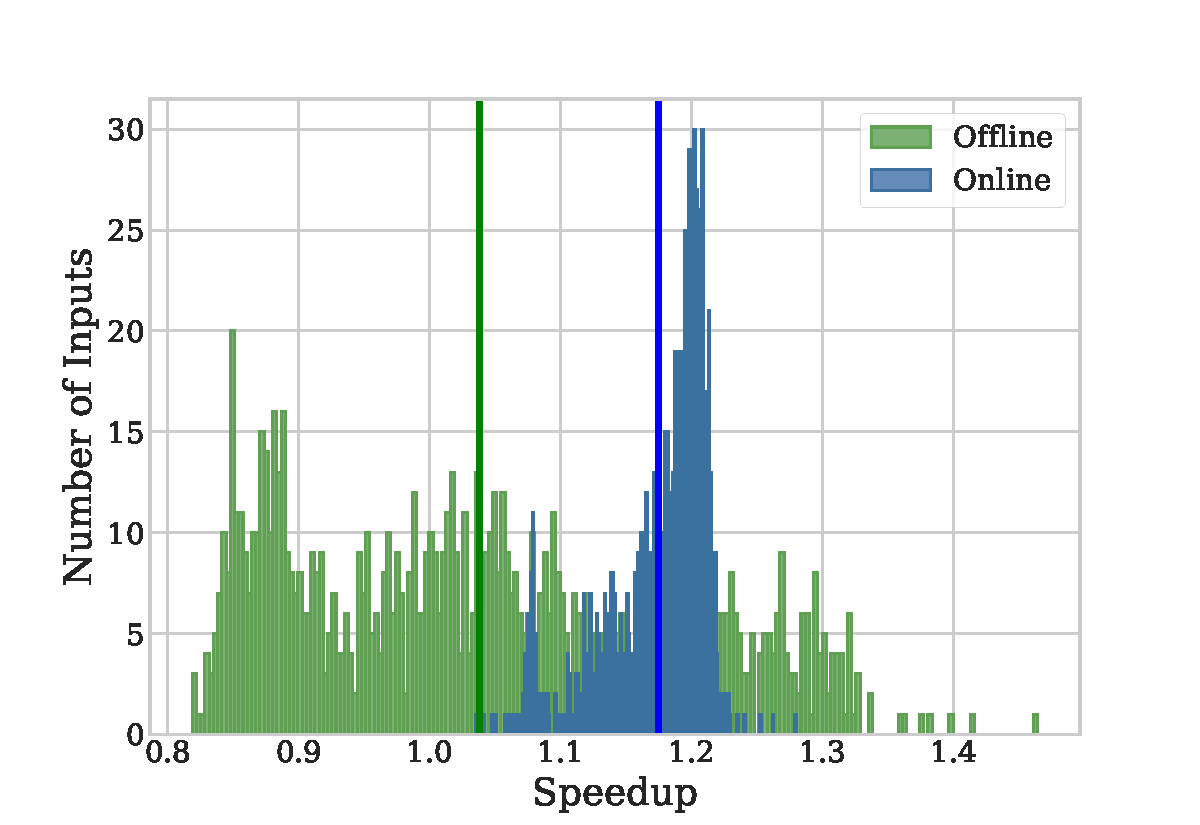
\includegraphics[width=0.5\textwidth]{figs/motivation-online.pdf}
%     \caption{Comparison between the offline and online {\itercomp}.
%              The vertical lines represent the average speedups over
%              all the 1,000 inputs.}
%     \label{fig:motivation-online}
% \end{figure}

% It is worth mentioning that our goal is to improve the average performance
% across the user's workload, and not only for a specific input.
% This means that the online {\itercomp} is better informed throughout the search,
% as it compares optimization sequences across different sets inputs.

% However, because of the restriction of having a single execution per input,
% it is not possible to measure speedup in a real-world online scenario.
% Moreover, measuring just execution time, for example, is also not viable since
% different inputs often mean different amounts of work,
% rendering it meaningless to compare optimizations only by execution time.
% Therefore, we need a performance metric which can be profiled from a single
% execution of the program.
% Although a previous work has suggested that \textit{instructions per cycle}~(IPC)
% could be used with that goal, IPC have no correlation with speedup~\citep{fursin07}.
% In a case where we have two distinct versions of the program, due to different
% optimizations, which is also executed with distinct inputs, higher IPC does not
% necessarily mean lower execution time (higher performance).
%
% \begin{figure}[t]
%     \centering
%     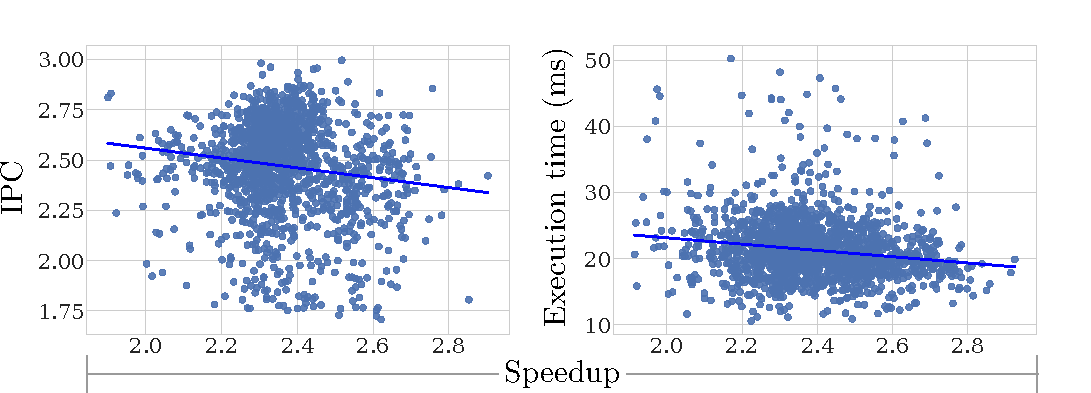
\includegraphics[width=0.5\textwidth]{figs/motivation-metric.pdf}
%     \caption{Comparison among different performance metrics for performing
%              online {\itercomp}.
%              The vertical lines represent the best score for each metric.}
%     \label{fig:motivation-metric}
% \end{figure}
%
% Figure~\ref{fig:motivation-metric} shows a comparison between execution time and IPC,
% and their correlation with the actual speedup.
% Each point in the figure corresponds to each metric averaged over
% a set of inputs, collected during the {\itercomp}.
% The vertical lines correspond to the optimization sequence
% with the best score for each one of the metrics.
% This figure shows that both execution time and IPC are unsuitable for
% online {\itercomp}, as they present no direct correlation with the actual
% speedup obtained by the optimization sequence being evaluated.
%
% In the remaining of this paper, we develop a work efficiency metric, suitable
% for guiding online {\itercomp}, which can be profiled with a single execution
% of the program with the optimization sequence being evaluated.
